\let\negmedspace\undefined
\let\negthickspace\undefined
\documentclass[journal]{IEEEtran}
\usepackage[a5paper, margin=10mm, onecolumn]{geometry}
%\usepackage{lmodern} 
\usepackage{tfrupee} 

\setlength{\headheight}{1cm} 
\setlength{\headsep}{0mm}     

\usepackage{gvv-book}
\usepackage{gvv}
\usepackage{cite}
\usepackage{amsmath,amssymb,amsfonts,amsthm}
\usepackage{algorithmic}
\usepackage{graphicx}
\usepackage{textcomp}
\usepackage{xcolor}
\usepackage{txfonts}
\usepackage{listings}
\usepackage{enumitem}
\usepackage{mathtools}
\usepackage{gensymb}
\usepackage{comment}
\usepackage[breaklinks=true]{hyperref}
\usepackage{tkz-euclide} 
\usepackage{listings}                                        
\def\inputGnumericTable{}                                 
\usepackage[latin1]{inputenc}                                
\usepackage{color}                                            
\usepackage{array}                                            
\usepackage{longtable}                                       
\usepackage{calc}                                             
\usepackage{multirow}                                         
\usepackage{hhline}                                           
\usepackage{ifthen}                                           
\usepackage{lscape}

\begin{document}

\bibliographystyle{IEEEtran}
\vspace{3cm}

\title{4.8.26}
\author{AI25BTECH11030 -Sarvesh Tamgade}
{\let\newpage\relax\maketitle}

\renewcommand{\thefigure}{\theenumi}
\renewcommand{\thetable}{\theenumi}
\setlength{\intextsep}{10pt} 


\numberwithin{equation}{enumi}
\numberwithin{figure}{enumi}
\renewcommand{\thetable}{\theenumi}


\textbf{Question}: Find the coordinates of the foot of the perpendicular drawn from the point
\[
\vec{P} = \myvec{2 \\ -3 \\ 4}
\]
to the \(Y\)-axis.

\textbf{Solution}:\
The \(Y\)-axis has the direction vector
\[
\vec{e_{2}} = \myvec{0 \\ 1 \\ 0}
\]
and passes through the origin. Its general point is
\[
\vec{Q} = \myvec{0 \\ q \\ 0}.
\]
Any point \(\vec{Q}\) on the \(Y\)-axis satisfies \(x = 0\) and \(z = 0\).

Let \(\vec{P} = \myvec{2 \\ -3 \\ 4}\).

The foot of the perpendicular \(\vec{Q}\) is given by projecting \(\vec{P}\) onto the \(Y\)-axis as
\[
\vec{Q} = \left(\vec{e_{2}}^\top \vec{P}\right) \frac{\vec{e_{2}}}{\|\vec{e_{2}}\|^2}.
\]


\[
\vec{e_{2}}^\top \vec{P} = \myvec{0 & 1 & 0} \myvec{2 \\ -3 \\ 4}.
\]

Since 
\[
\|\vec{e_{2}}\|^2 = 0^2 + 1^2 + 0^2 = 1,
\]
the foot of the perpendicular is
\[
\vec{Q} = \left( \myvec{0 & 1 & 0} \myvec{2 \\ -3 \\ 4} \right) \vec{e_{2}}.
\]

\[
\vec{Q} = (-3) \vec{e_{2}} = \myvec{0 \\ -3 \\ 0}.
\]

\textbf{Final Answer:} The coordinates of the foot of the perpendicular are
\[
\myvec{0 \\ -3 \\ 0}.
\]

\begin{figure}[htbp]
    \centering
    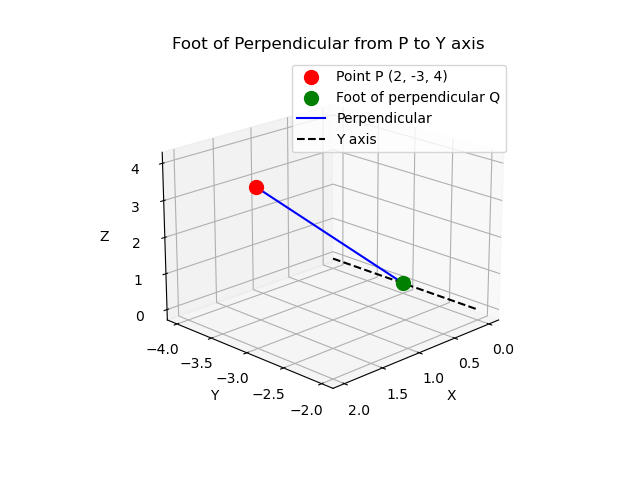
\includegraphics[width=0.65\linewidth]{FIG/fig1.png}
    \caption{Vector Representation}
    \label{fig:FIG/fig1.png}
    \end{figure}

\end{document}  